\section[\thesection \  Evaluierung]{Evaluierung}\label{sec:evaluation}

% Frame 10
\begin{frame}{Mean Average Precision (mAP)}
    \fontsize{9pt}{9pt}\selectfont
    \begin{columns}[T]
    \column{0.5\columnwidth}
    \textbf{\normalsize Intersection over Union (IoU)}
    \begin{figure}
        \centering
        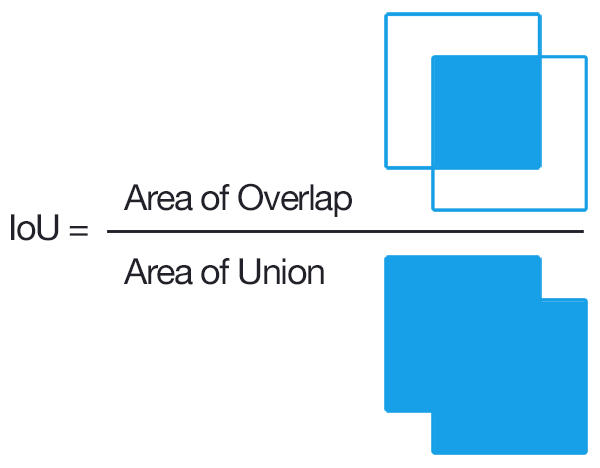
\includegraphics[width=0.7\textwidth]{Bilder/IoU.png}                    
    \end{figure}
    \begin{itemize}
        \item $\text{IoU} > 0.5 \rightarrow \textbf{True Positive}$
    \end{itemize}
    
    \column{0.5\columnwidth}
    \visible<2->{
    \textbf{Recall:} Trefferquote
    \begin{equation*}
        \frac{\text{True Positives}}{\text{alle Objekte im Bild}}
    \end{equation*}
    \\[0.2cm]
    \textbf{Precision} Genauigkeit 
    \begin{equation*}
        \frac{\text{True Positives}}{\text{alle Predictions}}
    \end{equation*}
    \\[0.2cm]
    \textbf{Average Precision} für eine Klasse
    \begin{equation*}
        AP = \frac{1}{N}\sum Precision(Recall)
    \end{equation*}
    }
    \end{columns}
    \visible<3->{
    \normalsize
    \begin{block}{Loss}
        \begin{itemize}
            \item \textbf{Lokalisierung:} Bounding Box Regression
            \item \textbf{Klassifizierung:} (Logarithmische) Fehlerberechnung
        \end{itemize}
        \vspace{0.3cm}
    \end{block}
    }
    
\end{frame}


% Frame 11
\begin{frame}{Auswirkung von Augmentierung}

    \begin{columns}[T]
        \column{0.05\textwidth}
        \vspace{1.5cm}
        Loss\\
        \vspace{3cm}
        mAP\\
        

        \column{0.45\textwidth}
        \centering
        Ohne Augmentierung
        \begin{figure}
            \centering
            \def\svgwidth{0.75\columnwidth}
            \footnotesize
            \input{Bilder/loss_ohne_aug.pdf_tex}
        \end{figure}

        \begin{figure}
            \centering
            \def\svgwidth{0.75\columnwidth}
            \footnotesize
            \input{Bilder/mAP_ohne_aug.pdf_tex}
        \end{figure}
        

        \column{0.45\textwidth}
        \centering
        Mit Augmentierung

        \begin{figure}
            \centering
            \def\svgwidth{0.75\columnwidth}
            \footnotesize
            \input{Bilder/loss_aug.pdf_tex}
        \end{figure}
        \begin{figure}
            \centering
            \def\svgwidth{0.75\columnwidth}
            \footnotesize
            \input{Bilder/mAP_aug.pdf_tex}
        \end{figure}
        
    \end{columns}
\end{frame}



\begin{frame}{Vergleich Modelle: Genauigkeit - Inferenzzeit}
    \begin{columns}
        \column{0.45\columnwidth}
        \textbf{Inferenzzeit}

% Please add the following required packages to your document preamble:
% \usepackage{multirow}
\begin{table}[]
    \begin{tabular}{|lccc|}
    \hline
    \multirow{2}{*}{\begin{tabular}[c]{@{}l@{}}Archi-\\ tecture\end{tabular}} & \multirow{2}{*}{\begin{tabular}[c]{@{}c@{}}Base\\ CNN\end{tabular}} & \multicolumn{2}{c|}{Infer FPS}                          \\
                                                                              &                                                                     & \multicolumn{1}{l}{Sync.} & \multicolumn{1}{l|}{Async.} \\ \hline
    \multirow{2}{*}{SSD}                                                      & Mobilenet                                                           & 12,6                      & 33,6                        \\
                                                                              & InceptionV2                                                         & 10,7                      & \textbf{28,3}               \\ \hline
    \multirow{2}{*}{\begin{tabular}[c]{@{}l@{}}Faster\\ R-CNN\end{tabular}}   & InceptionV2                                                         & 0,55                      & \textbf{0,72}               \\
                                                                              & ResNet50                                                            & -                         & -                           \\ \hline
    \end{tabular}
    \end{table}
        
        \column{0.1\columnwidth}
        \column{0.45\columnwidth}

        \visible<2->{
        \textbf{Genauigkeit}
        
        \begin{table}[]
            \begin{tabular}{|lll|}
            \hline
            Model                                                                                             & mAP                                                             & Loss                                                             \\ \hline
            \begin{tabular}[c]{@{}l@{}}SSD InceptionV2\\ +Augmentierung\end{tabular}                          & \begin{tabular}[c]{@{}l@{}}0.55\\ 0.6\end{tabular}              & \begin{tabular}[c]{@{}l@{}}4,4\\ 4,1\end{tabular}                \\ \hline
            \begin{tabular}[c]{@{}l@{}}Faster R-CNN\\ +Augmentierung\\ +Dropout\\ +L2 Regularis.\end{tabular} & \begin{tabular}[c]{@{}l@{}}0.67\\ 0.7\\ 0.7\\ adsf\end{tabular} & \begin{tabular}[c]{@{}l@{}}0.82\\ 0,7\\ 0.66\\ adfs\end{tabular} \\ \hline
            \end{tabular}
            \end{table}
        }
    \end{columns}
    
    \visible<3->{
    \begin{itemize}
        \centering
        \item Je genauer, desto langsamer!
    \end{itemize}
    }
    \end{frame}

% \begin{frame}{Modell Architektur} % ersetzen mit tabelle

%     \begin{columns}[T]
%         \column{0.05\textwidth}
%         \vspace{1.5cm}
%         Loss:
%         \\[2.2cm]
%         Inferenzzeit:

%         \column{0.45\textwidth}
%         \centering
%         SSD + InceptionV2
%         \begin{figure}
%             \centering
%             \def\svgwidth{0.8\columnwidth}
%             \tiny
%             \input{Bilder/loss_ssd.pdf_tex}
%         \end{figure}
%         \begin{itemize}
%             \centering
%             \item ca. $30ms$
%         \end{itemize}

%         \column{0.45\textwidth}
%         \centering
%         Faster RCNN + InceptionV2

%         \begin{figure}
%             \centering
%             \def\svgwidth{0.8\columnwidth}
%             \footnotesize
%             \input{Bilder/loss_aug.pdf_tex}
%         \end{figure}
%         \begin{itemize}
%             \centering
%             \item ca. $1000ms$
%         \end{itemize}
%     \end{columns}

%     \vspace{0.8cm}
%     \centering\large
%     Je genauer, desto langsamer die Inferenz!

% \end{frame}


